\chapter{Firewall}

For ACL, take a look at chapter ACL in Notebook folder.\\

\section{Background}

\subsection{Packet filtering}

Basic packet filtering firewalls can only filter based on Layer 3 and sometimes basic Layer 4 information. \\

\textbf{Benefits:} Cheap, Simple implementation, Low impact on network performance.\\

\textbf{Limitations:} Cannot prevent IP spoofing, Complex ACLs, \emph{Stateless} (examine each packet individually rather than in the context of the state of a connection).

\subsection{Statefull firewall}

Stateful firewall examine each packet in the context of the state of a connection. Stateful firewalls use a state table to keep track of the communication process.\\ 

\textbf{Benefits:} Prevent spoofing and DoS attacks.\\ 

\textbf{Limitations:} Cannot prevent UDP, ICMP, and layer 7 attacks; No authentication; Cannot detect dynamic port negotiation.

\subsection{DMZ}

A demilitarized zone (DMZ) is a firewall design where there is typically one inside interface connected to the private network, one outside interface connected to the public network, and one DMZ interfac. As shown in the figure \ref{DMZfilter}, all traffic towards internal network is denied, however, traffic originating from internal network can flow freely to other zones. Communication between the Internet and DMZ is selective permitted.\\

\begin{figure}[hbtp]
\caption{DMZ topology and traffic restriction}\label{DMZfilter}
\centering
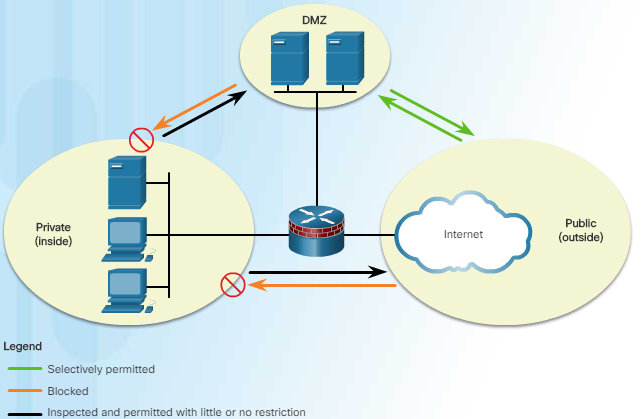
\includegraphics[width=10\xm]{pictures/DMZfilter.PNG}
\end{figure}

%\subsection{Layered Defense}
%
%A layered defense uses different types of firewalls that are combined in layers. Security policies can be enforced between the layers and inside the layers. A traffic from the untrusted network has to go through the following layers and policies:
%
%\begin{enumerate}
%\item Edge router (packet filtering)
%\item Bastion host (hardened computer located in the DMZ\footnote{This type of DMZ setup is called a \emph{screened subnet configuration}.}) or Screened firewall
%\item Interior screening router
%\end{enumerate}

\section{Classic firewall}\label{sec:ClassicFirewall}

Classic Firewall (CBAC) is a \emph{stateful} firewall that provides four main functions: Filtering, Inspection, Intrusion detection, and Generation of audits and alerts. It can only detects and protects against external attacks. The Classic Firewall applies firewall policy to interfaces.\\ 

Classic Firewall creates temporary ACE to allow returning traffic. These entries are created as inspected traffic leaves the network and are removed when the connection terminates or the idle timeout period for the connection is reached.\\

Take the topology in figure \ref{ClassicConfig} as an example for configuration. Suppose that the administrator wants to allow SSH sessions (in one direction) from 10.0.0.0/24 network to 172.30.0.0/24 network:

\begin{enumerate}
\item You have to define the internal and external interfaces. In this case, g0/0 is the inside and g0/1 is the outside interface.

\item Each interface is configured with an access list. The INSIDE access list for inside interface g0/0 allows only SSH traffic initiated from the 10.0.0.0/24 network. The OUTSIDE access list denies all traffic go into outside interface.

\item Next we define a rule FWRULE that inspect SSH connection originating from 10.0.0.0/24 network, then apply it to inside interface g0/0. With this rule, whenever an SSH communication is initiated from a host in 10.0.0.0/24 network, an ACE is created on the outside interface to allow the return SSH traffic go through the firewall.
\end{enumerate}

\begin{figure}[hbtp]
\caption{Network topology}\label{ClassicConfig}
\centering
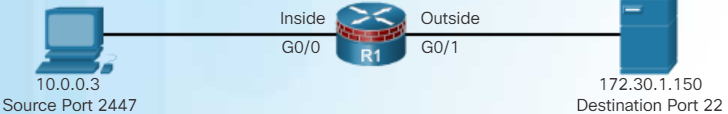
\includegraphics[width=10\xm]{pictures/ClassicConfig.PNG}
\end{figure}


\begin{sexylisting}{Classic Firewall configuration}
ip inspect name FWRULE ssh
ip access-list extended INSIDE
	permit tcp 10.0.0.0 0.0.0.255 any eq 22
	deny ip any any
	exit
ip access-list extended OUTSIDE
	deny ip any any
	exit	
int g0/0
	ip access-group INSIDE in
	ip inspect FWRULE in
	exit	
int g0/1
	ip access-group OUTSIDE in		
\end{sexylisting}

\section{Zone-based Policy Firewall (ZPF)}\label{sec:ZPF}

\subsection{Introduction}

Zone-Based Policy Firewall applies firewall policy to zones\footnote{A zone is a group of one or more interfaces.}. By default, the traffic between interfaces in the same zone passes freely. However, all zone-to-zone traffic is blocked or filtered by ZPF policies configured on each zone.\\

\textbf{Self zone} (the router itself) is a special zone that includes all the router interfaces. Any traffic is allowed to go through self-zone to reach another zone. Only packets destined to and sourced from the router (routing protocol messages, SSH packets, etc.) is restricted by policy.\\

An interface cannot belong to multiple zones. Traffic can never flow between an interface assigned to a zone and an interface without a zone assignment.\\

\tableStart[\caption{Compare Classic Firewall and ZPF operation}]{| p{6\xm} | p{2\xm} | p{2\xm} |}
\head{Content} & \head{Classic firewall} & \head{ZPF} \w
Only prevent attacks that travel through the firewall & $\bullet$ & \w
Require multiple ACLs and inspection actions &$\bullet$& \w
Not dependent on ACLs & & $\bullet$ \w
One policy affects any given traffic & & $\bullet$ \w
Firewall policy is applied on interfaces & $\bullet$ & \w
Firewall policy is applied on zones & & $\bullet$ \w
Examine connections for embedded NAT and PAT and perform address translation & $\bullet$ & \w
The default policy is to block unless explicitly allowed & & $\bullet$ \w
\tableEnd



\subsection{Configuration}

We need to enable Security Technology package before configuring ZPF. This can be done by using the command \code{license boot module c1900 technology-package securityk9}. After the enabling the package, save the running configuration and reload the router. Verify that the Security Technology package has been enabled by using the \code{show version} command.\\

Take the topology in figure \ref{ZPFtopology} as an example for configuration. The ZPF we are going to specify has to meet the following requirements:

\begin{itemize}
\item Traffic sourced from the PUBLIC zone and destined for the PRIVATE zone will only be allowed if it is part of sessions originally initiated by PRIVATE zone hosts.
\item Any HTTP, HTTPS, and DNS traffic from the PRIVATE zone to PUBLIC zone will be inspected. 
\end{itemize}


\begin{figure}[hbtp]
\caption{ZPF example topology}\label{ZPFtopology}
\centering
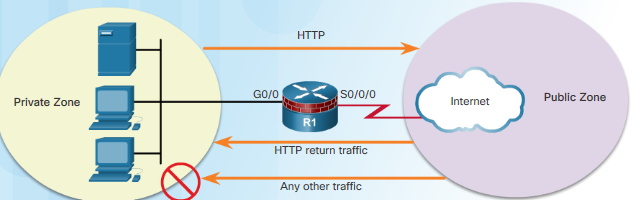
\includegraphics[scale=0.6]{pictures/ZPFtopology.PNG}
\end{figure}


\subsubsection{Step 1. Create a policy}
First of all, we need to specify which traffic between two zones we should inspect. To do this, we assign either pre-defined ACL or protocol port numbers or both to a class-map. In this example, all traffics originating from 192.168.3.0/24 network are defined in access list 100 and class-map PRIVATE-ACL-CLASS. Any traffic that utilizes HTTP, HTTPS, DNS protocol are assigned to the class-map PRIVATE-INTERNET-CLASS.\\

The next step is to create the policy that decides what to do witch each class-map. In this example, both class-maps we created are inspected.

\begin{sexylisting}{Create a ZPF policy}
access-list 100 permit ip 192.168.3.0 0.0.0.255 any
class-map type inspect match-all PRIVATE-ACL-CLASS
  match access-group 100    
class-map type inspect match-any PRIVATE-INTERNET-CLASS
  match protocol http
  match protocol https
  match protocol dns
exit    
policy-map type inspect PRIV-TO-PUB-POLICY
  class type inspect PRIVATE-ACL-CLASS   
  inspect    
  class type inspect PRIVATE-INTERNET-CLASS
  inspect
  class class-default
exit
\end{sexylisting}

There are three action available for dealing with each traffic

\begin{itemize}
\item \code{inspect} -- This action offers state-based traffic control. It tracks UDP or TCP connections and permit the return traffic.
\item \code{drop} -- This is the default action for all traffic. Similar to the implicit deny any at the end of every ACL, , there is an explicit \code{drop} applied to the end of every policy-map.
\item \code{pass} -- This action allows \emph{one-direction} traffic between two zones, and does not track the state of connections. A corresponding policy must be applied to allow return traffic to pass in the opposite direction. This action is ideal for secure protocols, such as IPsec. 
\end{itemize}

\subsubsection{Step 2. Create zones}
In this topology, we have two interfaces, two zones, and traffic flowing in one direction.
\begin{sexylisting}{Create zones}
zone security PRIVATE
zone security INTERNET
int g0/1
  zone-member security PRIVATE
int s0/0/0
  zone-member security INTERNET    
exit
\end{sexylisting}



\subsubsection{Step 3. Match zone pair and policy}
\begin{sexylisting}{Match zone pair and policy}
zone-pair security PRIVATE-2-INTERNET source PRIVATE destination INTERNET
  service-policy type inspect  PRIV-TO-PUB-POLICY
end
\end{sexylisting}



\subsubsection{Verification}

\begin{sexylisting}{ZPF Verification}
show run | begin class-map
show class-map type inspect
show zone security
show zone-pair security
show policy-map type inspect
show policy-map type inspect zone-pair sessions
\end{sexylisting}


%
%There are four steps to configure a ZPF zone (Take the topology in figure \ref{Zone} as an example):
%
%\begin{enumerate}
%\item \textbf{Create the zones and Assign zones to appropriate interfaces:} Associating a zone to an interface will immediately apply the service-policy that has been associated with the zone. If no service-policy is yet configured for the zone, all transit traffic will be dropped.
%
%\item \textbf{Identify traffic with class-map:} A class is a way of identifying a set of packets based on its contents using \code{match} conditions. Packets must meet one of the match criteria \code{match-any} or all of the match criteria \code{match-all} to be considered a member of the class. Table \ref{tab:classMap} shows the syntax for the \code{class-map} and its sub-commands.
%
%\item \textbf{Define an action with policy-map:} Assign class-maps defined in step 2 to a policy-map and define what action (Inspect, Drop, or Pass) should be taken for traffic that is a member of a class. 
%\item \textbf{Identify a zone-pair and match it to a policy-map:} 
%\end{enumerate}
%
%\begin{figure}[hbtp]
%\caption{ZPF configuration topology}\label{Zone}
%\centering
%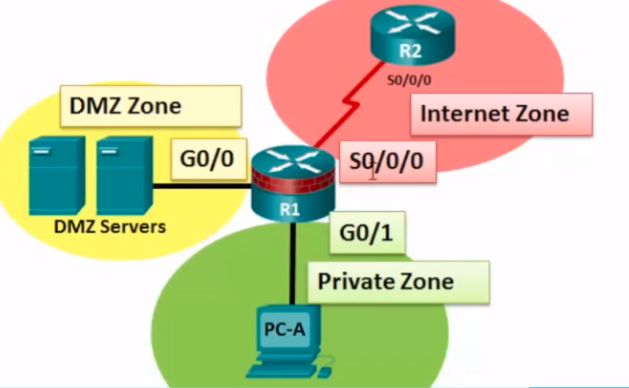
\includegraphics[scale=0.5]{pictures/Zone.PNG}
%\end{figure}
%
%\begin{sexylisting}{ZPF configuration}
%#STEP 1
%zone security PRIVATE
%zone security INTERNET
%zone security DMZ
%int g0/1
%  zone-member security PRIVATE
%int s0/0/0
%  zone-member security INTERNET    
%int g0/0
%  zone-member security DMZ
%exit
%
%#STEP 2
%class-map type inspect match-all PRIVATE-ACL-CLASS
%  match access-group 100    
%class-map type inspect match-any PRIVATE-INTERNET-CLASS
%  match protocol http
%  match protocol https
%  match protocol dns
%exit    
%
%#STEP 3
%policy-map type inspect PRIV-TO-PUB-POLICY
%  class type inspect PRIVATE-ACL-CLASS   
%  inspect    
%  class type inspect PRIVATE-INTERNET-CLASS
%  inspect
%  class class-default
%exit   
%
%#STEP 4
%zone-pair security PRIVATE-2-INTERNET source PRIVATE destination INTERNET
%  service-policy type inspect  PRIV-TO-PUB-POLICY
%end
%\end{sexylisting}

%\subsection{Command syntax and some considerations}
%
%\begin{itemize}
%\item An interface cannot belong to multiple zones.
%ZPF can coexist with Classic Firewall although they cannot be used on the same interface. Remove the \code{ip inspect} interface configuration command before applying the \code{zone-member security} command.
%\item Traffic can never flow between an interface assigned to a zone and an interface without a zone assignment. Applying the zone-member configuration command always results in a temporary interruption of service until the other zone-member is configured.
%\item Communication between zones are, by default, dropped. Unless there exits a service-policy configured for the zone-pair.
%\item The \code{zone-member} command does not protect the router itself (traffic to and from the router is not affected) unless the zone-pairs are configured using the predefined self zone.
%\end{itemize}
%
%\tableStart[\caption{The syntax of class-map command}\label{tab:classMap}] { |p{5\xm}|p{8\xm}| }
%\multicolumn{2}{|c|}{ \code{class-map type inspect [match-any | match-all] <class-name>} } \w
%\head{Parameter}&\head{Description} \w
%\code{match-any} & Packets must meet one of the criteria to be considered a member of the class.\w
%\code{match-all} & Packets must meet all of the criteria to be considered a member of the class.\w
%\code{match protocol <protocol-name>} & Configure criteria based on specified protocol.\w
%\code{match access-group <acl-name>} & Configure criteria based on specified ACL.\w
%\code{match class-map <class-name>} & Use another class-map as criteria.\w
%\tableEnd


